% Complete Master CV -- source of truth, not a one-page job application
% Retains the original TU Wien Overleaf style.tex and photo convention.
%-------------------------
% ATS-Friendly Resume Style
% Keep this file unchanged when tailoring your CV.
%-------------------------

\documentclass[letterpaper,11pt]{article}

%---------- PACKAGES ----------
\usepackage{latexsym}
\usepackage[empty]{fullpage}
\usepackage{titlesec}
\usepackage[dvipsnames]{xcolor}
\usepackage{enumitem}
\usepackage[hidelinks]{hyperref}
\usepackage{fancyhdr}
\usepackage[english]{babel}
\usepackage{tabularx}



%---------- FONT ----------
% Same font family and weight as the original template
\usepackage{iftex}
\usepackage{graphicx}
\ifPDFTeX
  % pdfLaTeX-safe, selectable text and a close Arial-like font.
  \usepackage[T1]{fontenc}
  \usepackage[utf8]{inputenc}
  \usepackage[scaled=0.96]{helvet}
  \renewcommand{\familydefault}{\sfdefault}
  \input{glyphtounicode}
  \pdfgentounicode=1
\else
  % Keep the original Arimo typography under XeLaTeX / LuaLaTeX.
  \usepackage{fontspec}
  \IfFontExistsTF{Arimo}{
    \setmainfont{Arimo}
    \setsansfont{Arimo}
    \setmonofont{Arimo}
  }{
    \setmainfont{TeX Gyre Heros}
    \setsansfont{TeX Gyre Heros}
    \setmonofont{Latin Modern Mono}
  }
\fi
\newcommand{\cvsemibold}{\bfseries}
\definecolor{europassblue}{HTML}{4E9DCE}
\definecolor{cvgray}{HTML}{1A1A1A}

%---------- ATS / PDF TEXT EXTRACTION ----------

\hypersetup{
  pdfauthor={Muhammad Asad},
  pdftitle={Muhammad Asad - CV},
  pdfsubject={Resume},
  pdfkeywords={}
}

%---------- PAGE STYLE ----------
\pagestyle{fancy}
\fancyhf{}
\fancyfoot{}
\renewcommand{\headrulewidth}{0pt}
\renewcommand{\footrulewidth}{0pt}

%---------- MARGINS ----------
\addtolength{\oddsidemargin}{-0.5in}
\addtolength{\evensidemargin}{-0.5in}
\addtolength{\textwidth}{1in}
\addtolength{\topmargin}{-0.5in}
% Shift the complete CV upward by 28pt without changing internal spacing.
\addtolength{\topmargin}{-18pt}
\addtolength{\textheight}{1.0in}

\urlstyle{same}
\color{black}
\raggedbottom
\raggedright
\setlength{\tabcolsep}{0in}
\setlength{\parindent}{0pt}

%---------- SECTION FORMATTING ----------
\titleformat{\section}
  {\vspace{-4pt}\color{black}\bfseries\raggedright\large}
  {}{0em}{}
  [\color{europassblue}\titlerule\vspace{-5pt}]

%---------- CUSTOM COMMANDS ----------
\newcommand{\resumeItem}[1]{
  \item\small{#1}
}

\newcommand{\resumeSubheading}[4]{
  \vspace{-2pt}\item
  \begin{tabular*}{0.97\textwidth}[t]{l@{\extracolsep{\fill}}r}
    {\small\cvsemibold\color{cvgray} #1} & {\small #2} \\
    \textit{\small #3} & \textit{\small #4} \\
  \end{tabular*}\vspace{-7pt}
}

\newcommand{\resumeProjectHeading}[2]{
  \item
  \begin{tabular*}{0.97\textwidth}[t]{l@{\extracolsep{\fill}}r}
    \small\color{cvgray} #1 & #2 \\
  \end{tabular*}\vspace{-7pt}
}

\renewcommand\labelitemii{$\vcenter{\hbox{\tiny$\bullet$}}$}

\newcommand{\resumeSubHeadingListStart}{\begin{itemize}[leftmargin=0.15in,label={}]}
\newcommand{\resumeSubHeadingListEnd}{\end{itemize}}
\newcommand{\resumeItemListStart}{\begin{itemize}[leftmargin=0.38in, itemsep=2pt, parsep=0pt, topsep=3pt, partopsep=0pt]}
\newcommand{\resumeItemListEnd}{\end{itemize}\vspace{-5pt}}

% Europass-inspired single-line work heading: role -- company -- dates -- location
\newenvironment{experienceblock}[4]{%
  \par\vspace{5pt}\noindent
  {\small\color{cvgray}{\cvsemibold #1 -- #2} -- #3 -- #4}\par\vspace{1pt}
}{\par\vspace{3pt}}

\begin{document}
\vspace*{-16pt}
\noindent
\begin{minipage}[t]{0.19\textwidth}
  \vspace{0pt}
  \IfFileExists{pic_refined.png}{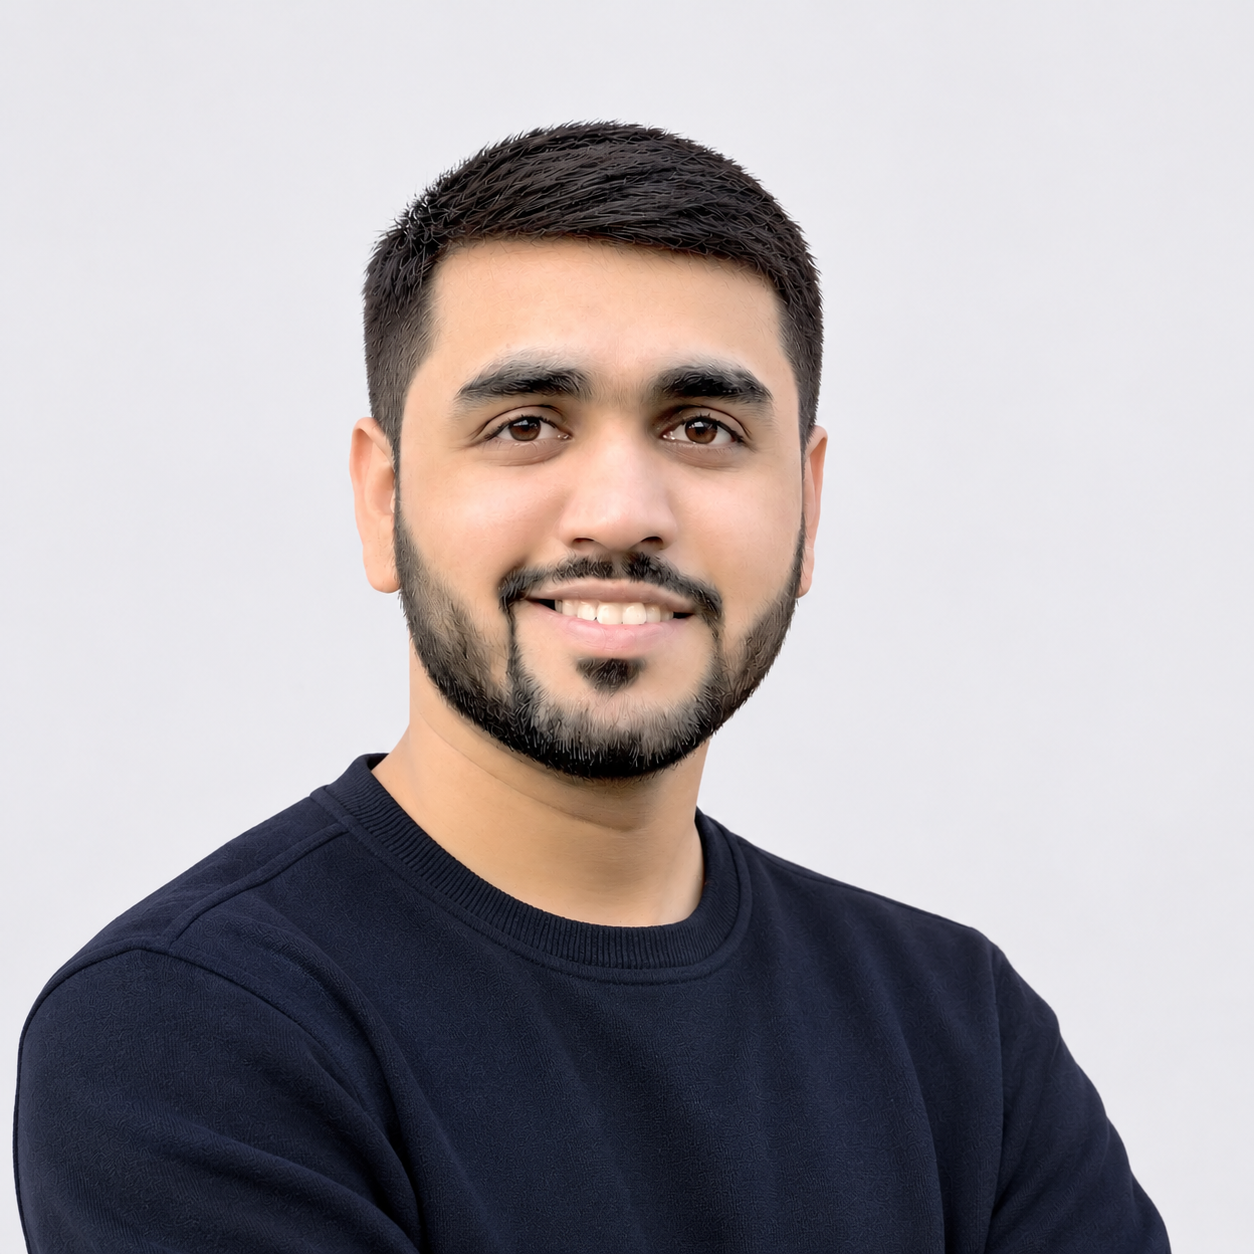
\includegraphics[width=\linewidth,height=2.65cm,keepaspectratio]{pic_refined.png}}{\rule{0pt}{2.65cm}}
\end{minipage}\hfill
\begin{minipage}[t]{0.77\textwidth}
  \vspace{0pt}\raggedright
  {\fontsize{23}{27}\selectfont\bfseries\color{europassblue} Muhammad Asad}\par\vspace{7pt}
  {\small +43 677 64100047 \quad $|$ \quad \href{mailto:muhammad.asad5152@gmail.com}{muhammad.asad5152@gmail.com}}\par\vspace{4pt}
  {\small \href{https://github.com/asad-arif}{github.com/asad-arif} \quad $|$ \quad \href{https://linkedin.com/in/mdotasad}{linkedin.com/in/mdotasad}}\par\vspace{4pt}
  {\small Vienna, Austria \quad $|$ \quad MSc Data Science, TU Wien}
\end{minipage}
\par\vspace{5pt}

\section{Profile}

\noindent{\small Software Engineer and MSc Data Science student at TU Wien with experience across AI-enabled applications, RAG and LLM integrations, knowledge graphs, data pipelines, full-stack web development, and interactive 3D products. Experienced in building user-facing applications, backend APIs, and cloud-deployed systems using Python, JavaScript/TypeScript, React, Next.js, Three.js, and AWS.}\par\vspace{3pt}

\section{Work Experience}

\par\vspace{4pt}\noindent{\small\bfseries Software Engineer | Devfum | Lahore, Pakistan | Aug 2024 -- Feb 2026}\par

\noindent{\small Built AI-enabled product features using LLM APIs and LangChain, including functionality supporting architectural material cost estimation.}\par\vspace{2pt}

\noindent{\small Developed interactive 3D product configurators and e-commerce experiences with Three.js, React Three Fiber, React, and Next.js.}\par\vspace{2pt}

\noindent{\small Contributed to the Duncan packaging configurator and immersive 3D commerce products, including product presentation and customization workflows.}\par\vspace{2pt}

\noindent{\small Implemented frontend interfaces, backend APIs, authentication and database integrations for full-stack applications.}\par\vspace{2pt}

\noindent{\small Worked with AWS services, deployment workflows, CI/CD, testing, and code reviews.}\par\vspace{2pt}

\noindent{\small Worked on 3D rendering materials, model loading, and interactive product visualization.}\par\vspace{2pt}

\par\vspace{4pt}\noindent{\small\bfseries Associate Software Engineer | SprintX | Lahore, Pakistan | Sep 2023 -- May 2024}\par

\noindent{\small Developed Crosscheck QA platform features, including test cases, test runs, bug reporting, user roles, and administrative workflows.}\par\vspace{2pt}

\noindent{\small Integrated workflows involving a Chrome extension and external tools including Jira and ClickUp.}\par\vspace{2pt}

\noindent{\small Contributed features, bug fixes, and responsive interfaces across multiple Oplii enterprise asset management modules.}\par\vspace{2pt}

\noindent{\small Improved the SprintX website Lighthouse performance score from approximately 60 to 90 through performance and SEO improvements.}\par\vspace{2pt}

\noindent{\small Collaborated with QA engineers and developers on implementation, debugging, and delivery.}\par\vspace{2pt}

\par\vspace{4pt}\noindent{\small\bfseries Software Engineer Intern | Softrixtech | Jun 2021 -- Aug 2021}\par

\noindent{\small Developed React task-management and e-commerce applications using Hooks, Context API, REST APIs, CRUD operations and reusable components.}\par\vspace{2pt}

\par\vspace{4pt}\noindent{\small\bfseries Freelance Software Engineer | Fiverr | From Jun 2019 (historical; end date not confirmed)}\par

\noindent{\small Delivered freelance web/software development services for international clients; achieved Level Two Seller status. Historical project and client counts require verification.}\par\vspace{2pt}

\section{Project Inventory}

\par\vspace{4pt}\noindent{\small\bfseries Formula 1 Knowledge Graph \& Analytics | Python, Neo4j, PyKEEN, Streamlit}\par

\noindent{\small Built an F1 ETL pipeline covering 1950--2025 with 47,208 nodes and 92,189 relationships; normalized and batch-imported graph entities; built Streamlit analytics and evaluated TransE, ConvE and ComplEx embeddings.}\par\vspace{2pt}

\par\vspace{4pt}\noindent{\small\bfseries Award-Winning RAG Application | PUCON, Lahore}\par

\noindent{\small Developed a retrieval-augmented generation application as part of a winning competition project; retrieval and LLM-based answer generation.}\par\vspace{2pt}

\par\vspace{4pt}\noindent{\small\bfseries Duncan | Interactive 3D Packaging Configurator}\par

\noindent{\small Developed a product customization experience with real-time 3D packaging previews for brand-specific packaging before printing.}\par\vspace{2pt}

\par\vspace{4pt}\noindent{\small\bfseries Hemero | Full-Stack 3D Product Application | \href{https://hemero.team/}{hemero.team/}}\par

\noindent{\small Contributed to an end-to-end 3D application spanning interactive frontend, backend functionality and deployment.}\par\vspace{2pt}

\par\vspace{4pt}\noindent{\small\bfseries Strikeo | 3D Multi-Vendor E-Commerce | \href{https://strikeo.com/}{strikeo.com/}}\par

\noindent{\small Developed a 3D e-commerce platform with interactive virtual plaza and product shopping experiences.}\par\vspace{2pt}

\par\vspace{4pt}\noindent{\small\bfseries Crosscheck | QA Management Platform | SprintX}\par

\noindent{\small Built workflows for test cases, bug reports, tickets, users and workspaces; supported Jira/ClickUp integrations and Chrome extension workflows.}\par\vspace{2pt}

\par\vspace{4pt}\noindent{\small\bfseries Oplii | Enterprise Asset Management | SprintX}\par

\noindent{\small Contributed to asset inspections, work orders, responsive workflows, offline synchronization and location-related features.}\par\vspace{2pt}

\par\vspace{4pt}\noindent{\small\bfseries Semantic Search API | Python, FastAPI, FAISS}\par

\noindent{\small Developed embedding and similarity-search endpoints using sentence-transformers and FAISS, with application/backend integrations.}\par\vspace{2pt}

\par\vspace{4pt}\noindent{\small\bfseries Amazon Reviews Classification | Apache Spark}\par

\noindent{\small Worked with large-scale review data using Spark RDD, SQL and MLlib, including multiclass classification and model tuning.}\par\vspace{2pt}

\par\vspace{4pt}\noindent{\small\bfseries Formula 1 Interactive Visualization | Plotly}\par

\noindent{\small Designed visual exploration of F1 practice, qualifying and race sessions, circuits and seasons.}\par\vspace{2pt}

\par\vspace{4pt}\noindent{\small\bfseries CIA Factbook Data Visualization | R, Plotly}\par

\noindent{\small Analyzed education spending, youth unemployment, migration and regional development categories using statistical and interactive visualizations.}\par\vspace{2pt}

\par\vspace{4pt}\noindent{\small\bfseries Swiss3D | \href{https://swiss3d.ch/en}{swiss3d.ch/en}}\par

\noindent{\small Historical portfolio association; individual contributions not yet documented. Retained for reference rather than claimed as a completed project.}\par\vspace{2pt}

\par\vspace{4pt}\noindent{\small\bfseries SyncMate and Biohy | Historical projects}\par

\noindent{\small Analytics dashboard and e-commerce frontend work; project dates and attribution not confirmed.}\par\vspace{2pt}

\par\vspace{4pt}\noindent{\small\bfseries Hostel Management System | Java, NetBeans}\par

\noindent{\small Object-oriented programming coursework project.}\par\vspace{2pt}

\section{Research Experience}

\par\vspace{4pt}\noindent{\small\bfseries Research Assistant | University of Education, Faisalabad Campus | Feb 2022 -- May 2023 (historical dates)}\par

\noindent{\small Supported NLP research on healthcare patient feedback (Care Opinion), including literature reviews, data organization and research documentation. An older CV used the title Teaching Assistant; this is treated as one appointment, not two.}\par\vspace{2pt}

\par\vspace{4pt}\noindent{\small\bfseries Bachelor's Thesis | Digital Infrared Thermal Imaging for Breast Cancer Screening | Oct 2022 -- May 2023}\par

\noindent{\small Advisor: Mr. Fahad Anwaar. Preprocessed thermal-image data, extracted features and trained classification models; reported 98.75\% project accuracy. Dataset, validation method and clinical generalizability have not been independently established.}\par\vspace{2pt}

\section{Education}

\par\vspace{4pt}\noindent{\small\bfseries MSc Data Science | Technische Universität Wien | Mar 2026 -- Present}\par

\noindent{\small Relevant work: data-intensive computing, machine learning, knowledge graphs, information visualization and analytics.}\par\vspace{2pt}

\par\vspace{4pt}\noindent{\small\bfseries BSc Information Technology | University of Education, Lahore | Nov 2019 -- Jul 2023}\par

\noindent{\small CGPA 3.70/4.00. Coursework: AI, Data Mining, Data Structures, OOP, Web Programming, Databases, Cloud Computing and Networking.}\par\vspace{2pt}

\par\vspace{4pt}\noindent{\small\bfseries Intermediate in Computer Science | Government Degree College Pasrur | Sep 2017 -- Jun 2019}\par

\par\vspace{4pt}\noindent{\small\bfseries 742/1100 marks. Matriculation in Computer Science | Government High School Ban Bajwa | 2015--2017 | 888/1100.}\par

\section{Technical Skills}

\noindent{\small AI / ML: LLM APIs, RAG, LangChain, LangGraph, knowledge graphs, PyKEEN, scikit-learn, embeddings, FAISS, sentence-transformers}\par\vspace{3pt}

\noindent{\small Data / Analytics: Python, SQL, pandas, Apache Spark (RDD, SQL, MLlib), ETL, Neo4j, Cypher, Streamlit, Plotly, R, Matplotlib}\par\vspace{3pt}

\noindent{\small Frontend / 3D: JavaScript, TypeScript, HTML, CSS, React, Next.js, Three.js, React Three Fiber, Redux, Tailwind, Sass/SCSS, Bootstrap, Vite, Figma}\par\vspace{3pt}

\noindent{\small Backend / Databases: Node.js, Express, REST APIs, MongoDB, PostgreSQL, MySQL, FastAPI, authentication/JWT}\par\vspace{3pt}

\noindent{\small Cloud / Tools: AWS, Docker, CI/CD, Git, GitHub, Postman, Swagger, Vercel, Netlify}\par\vspace{3pt}

\noindent{\small Concepts: OOP, data structures, MVC, API design, responsive UI, debugging, performance optimization}\par\vspace{3pt}

\noindent{\small Additional research tools: OpenCV, MATLAB, NumPy, NLTK, image processing, feature engineering, C/C++ and Java.}\par\vspace{3pt}

\section{Awards \& Achievements}

\noindent{\small PUCON Lahore --- Winning RAG application project (competition title/year to confirm).}\par\vspace{3pt}

\noindent{\small SprintX --- Developer of the Month (2024).}\par\vspace{3pt}

\noindent{\small University of Education --- Department top position holder / highest CGPA recognition (2024).}\par\vspace{3pt}

\noindent{\small University of Education / PEEF --- Merit-based PEEF Scholarship / tuition support for four semesters (reported; exact award wording and dates to verify).}\par\vspace{3pt}

\noindent{\small ICP 2022 --- Recognition for IT services and project management at an international science innovation conference.}\par\vspace{3pt}

\noindent{\small Prime Minister Laptop Scheme --- Laptop award for academic performance (2017).}\par\vspace{3pt}

\noindent{\small Fiverr --- Level Two Seller; served 300+ clients (self-reported).}\par\vspace{3pt}

\noindent{\small Outstanding Undergraduate Research Award (2023), University of Education --- as reported on LinkedIn; evidence pending.}\par\vspace{3pt}

\noindent{\small Floriculture Exhibition Competition --- First Position (historical; year not confirmed).}\par\vspace{3pt}

\section{Certifications \& Evidence}

\noindent{\small IBM --- Python for Data Science, AI \& Development  \href{https://www.coursera.org/account/accomplishments/verify/79WY2FE3Q6W7}{www.coursera.org/account/accomplishments/verify/79WY2FE3Q6W7}}\par\vspace{3pt}

\noindent{\small University of Michigan --- Programming for Everybody  \href{https://www.coursera.org/account/accomplishments/verify/FSAD69YNKQ59}{www.coursera.org/account/accomplishments/verify/FSAD69YNKQ59}}\par\vspace{3pt}

\noindent{\small University of California --- Work Smarter, Not Harder  \href{https://www.coursera.org/account/accomplishments/verify/X5NXXDL29D4L}{www.coursera.org/account/accomplishments/verify/X5NXXDL29D4L}}\par\vspace{3pt}

\noindent{\small Simplilearn --- HTML  \href{https://drive.google.com/file/d/1kQSFdofR6HyqfbHq_L8HAr9A4z3SFI0j/view?usp=sharing}{drive.google.com/file/d/1kQSFdofR6HyqfbHq\_L8HAr9A4z3SFI0j/view?usp=sharing}}\par\vspace{3pt}

\noindent{\small Simplilearn --- CSS  \href{https://drive.google.com/file/d/1dz-Xb_eHKpRmX9-eFCjIOJ96f7p2tj7x/view?usp=drive_link}{drive.google.com/file/d/1dz-Xb\_eHKpRmX9-eFCjIOJ96f7p2tj7x/view?usp=drive\_link}}\par\vspace{3pt}

\noindent{\small Simplilearn --- JavaScript  \href{https://drive.google.com/file/d/1bDhF5ksEw9lk6r5lVVllwjufzNDEko3L/view?usp=sharing}{drive.google.com/file/d/1bDhF5ksEw9lk6r5lVVllwjufzNDEko3L/view?usp=sharing}}\par\vspace{3pt}

\noindent{\small ICP 2022 --- IT Services Award  \href{https://drive.google.com/file/d/1JdLshTa870T2N9Z1CDxWyd97Jv-uMByq/view?usp=sharing}{drive.google.com/file/d/1JdLshTa870T2N9Z1CDxWyd97Jv-uMByq/view?usp=sharing}}\par\vspace{3pt}

\noindent{\small Meta Front-End Developer (Coursera): historical record lists this as ongoing; completion unconfirmed.}\par\vspace{3pt}

\section{Languages \& Volunteering}

\noindent{\small Urdu --- Native | English --- Professional | Punjabi --- Full professional | German --- Beginner}\par\vspace{3pt}

\noindent{\small UE Blood Society; Ijaz Noori Foundation Welfare Society; ICP 2022 conference IT infrastructure support (historical volunteer activities).}\par\vspace{3pt}

\section{Academic References}

\noindent{\small Mr. Fahad Anwaar | Lecturer and thesis advisor | University of Education | fahad.anwar@ue.edu.pk}\par\vspace{3pt}

\noindent{\small Dr. Nazia Anwar | IT Department Coordinator | University of Education | nazia.anwar@ue.edu.pk}\par\vspace{3pt}

\noindent{\small Dr. Muhammad Anwar | Assistant Professor | University of Education | anwar.muhammad@ue.edu.pk (email unverified; do not contact without confirmation)}\par\vspace{3pt}

\section{Portfolio \& Supporting Sources}

\noindent{\small Hemero  \href{https://hemero.team/}{hemero.team/}}\par\vspace{3pt}

\noindent{\small Strikeo  \href{https://strikeo.com/}{strikeo.com/}}\par\vspace{3pt}

\noindent{\small Swiss3D  \href{https://swiss3d.ch/en}{swiss3d.ch/en}}\par\vspace{3pt}

\noindent{\small LinkedIn  \href{https://www.linkedin.com/in/mdotasad/}{www.linkedin.com/in/mdotasad/}}\par\vspace{3pt}

\noindent{\small GitHub  \href{https://github.com/asad-arif}{github.com/asad-arif}}\par\vspace{3pt}

\section{Internal Verification Notes (Not for Applications)}

\noindent{\small Research role is recorded as Research Assistant; older source says Teaching Assistant. Confirm official appointment title and dates if a certificate is available.}\par\vspace{3pt}

\noindent{\small Dr. Muhammad Anwar's email was supplied separately and conflicts with an older CV that duplicated Dr. Nazia Anwar's email. Verify before sharing externally.}\par\vspace{3pt}

\noindent{\small Fiverr 300+ clients and 450+ projects are historical self-reported figures, not equivalent measures; no numerical claim used in the main experience section.}\par\vspace{3pt}

\noindent{\small Meta certification completion, research award, PUCON award details, project attribution (especially Swiss3D), and some historic dates require supporting evidence.}\par\vspace{3pt}

\noindent{\small This is a comprehensive master record, not a job-specific CV. Omit the internal notes and unverified claims when tailoring applications.}\par\vspace{3pt}

\section{Additional Project Detail}

\noindent{\small Formula 1 Knowledge Graph: ETL, normalized graph entities, validated imports and embedding evaluation across TransE, ConvE and ComplEx; 1950--2025 data coverage.}\par\vspace{3pt}

\noindent{\small Crosscheck QA: Chrome extension supporting network capture, screenshots and screen recording; test cases, test runs, bug assignments, workspaces, user roles and Jira/ClickUp integrations.}\par\vspace{3pt}

\noindent{\small Oplii EAM: asset inspections, work orders, offline synchronization and responsive enterprise workflows.}\par\vspace{3pt}

\noindent{\small Duncan: 3D packaging previews, NextAuth sessions and JWT-based authentication, real-time product customization.}\par\vspace{3pt}

\noindent{\small Strikeo: Next.js, Three.js, Tailwind CSS, NextAuth, Redux Toolkit Query and Vercel; catalog, search, filtering, sorting, shopping cart and interactive 3D plaza.}\par\vspace{3pt}

\noindent{\small Semantic Search API: Python FastAPI, FAISS, sentence-transformers, MongoDB Atlas and Node.js server-side integration.}\par\vspace{3pt}

\noindent{\small Amazon Reviews: approximately 12 million reviews across 23 categories; Spark RDD, Spark SQL and MLlib; multiclass classification and tuning, with 80/20 split and seed 42 in coursework.}\par\vspace{3pt}

\noindent{\small CIA Factbook 2020: education expenditure (\% GDP), youth unemployment (15--24), net migration, development status and continent/subcontinent; density, bar, mosaic, box, scatter, parallel coordinates, world map and Plotly.}\par\vspace{3pt}

\noindent{\small Hemero: interactive 3D frontend, full-stack backend and deployment; project link retained in portfolio section.}\par\vspace{3pt}

\section{Additional Academic Detail}

\noindent{\small Bachelor thesis proposed rural-access screening support, hospital referrals and first-aid suggestions. Expansion of datasets, security and automated reminders were described as future plans, not completed features.}\par\vspace{3pt}

\noindent{\small Bachelor thesis reported 98.75\% classification accuracy on project experiments; this is not a clinically validated diagnostic performance claim.}\par\vspace{3pt}

\noindent{\small University of Michigan Python course: Feb--Jul 2023, reported grade 98.25\%. IBM Python for Data Science, AI \& Development: Mar--Jul 2023, reported grade 94.13\%.}\par\vspace{3pt}

\noindent{\small Intermediate in Computer Science: Government Degree College Pasrur, 742/1100. Matriculation in Computer Science: Government High School Ban Bajwa, 888/1100.}\par\vspace{3pt}

\section{Additional Professional Detail}

\noindent{\small Fiverr historical academic CV: Level Two Seller since June 2019; claimed team delivery of 450+ projects, 4.9 rating and 100\% satisfaction. Separate later claim of 300+ clients. Counts and current status not independently verified.}\par\vspace{3pt}

\noindent{\small Freelance activities described as web development, design, marketing and business-development services with an international client base; historical CV reports coordinating a team.}\par\vspace{3pt}

\section{Additional Skills Detail}

\noindent{\small Further self-reported technologies: React Hook Form, Formik/Yup, Material UI, RTK Query, Axios, Storybook, shadcn/ui, Angular, Three.js drei, GLTF/GLB, HDRI, SkeletonUtils, useGraph, AWS Lambda, API Gateway, DynamoDB and EC2.}\par\vspace{3pt}

\noindent{\small Further research interests: NLP, information retrieval, text mining, recommender systems, predictive analytics, health informatics, computer vision and machine learning.}\par\vspace{3pt}

\section{Additional Achievement Detail}

\noindent{\small University of Education: department top position holder; scholarship described in sources as full tuition fee waiver / PEEF merit support for four semesters; precise scholarship classification to confirm.}\par\vspace{3pt}

\noindent{\small ICP 2022: contributed IT infrastructure for an international conference at University of Education and received an IT services award (evidence link in certifications section).}\par\vspace{3pt}

\noindent{\small Floriculture Exhibition Competition: first position. Prime Minister Laptop Scheme: reported laptop award in 2017.}\par\vspace{3pt}

\section{Additional Volunteer Detail}

\noindent{\small University of Education Blood Society: blood donation activities. Ijaz Noori Foundation Welfare Society: volunteer member. ICP 2022: conference IT infrastructure.}\par\vspace{3pt}

\section{Historical Contact and Identity Record}

\noindent{\small Previous Pakistan contact emails and telephone numbers are intentionally not used for applications; current Vienna details are authoritative. Earlier GitHub username mdotasad and current github.com/asad-arif should not be conflated.}\par\vspace{3pt}

\section{Evidence Still Needed}

\noindent{\small Employment letters; TU Wien enrolment and transcripts; BSc transcript; thesis report/results; scholarship certificate; PUCON award; Outstanding Undergraduate Research Award; Fiverr profile; Swiss3D role evidence; Meta certification completion.}\par\vspace{3pt}

\noindent{\small Three referees retained above. Dr. Muhammad Anwar email is unverified due to a duplicated email in the historical academic CV; seek consent and confirm before contacting.}\par\vspace{3pt}

\noindent{\small University research appointment is recorded under the single working title Research Assistant (Feb 2022--May 2023); historical source also used Teaching Assistant. Do not represent these as two positions.}\par\vspace{3pt}

\end{document}